\chapter{Introduction}

Fluids are a vital part of everyday life - two of the most common ones being the air we breath and the water we drink. Less obvious are all the ways even these common fluids function behind the scenes in our day to day activities. Water, for example, serves an important role in various industrial settings, proving useful in areas ranging from thermal management to energy production; steam turbines alone accounted for 45\% of electricity generation in the United States in 2021 \cite{US_elec_gen_stat}. Improvements to these types of systems impact technologies across a variety of fields and are thus an important area of research. One strategy toward this end, and the primary motivator of the work presented here, is the use of supercritical fluids as the working fluid of these systems.  

In order to discuss supercritical fluids further, we must first go into more detail about general fluids. A \textit{fluid} is a large collection of mutually interacting particles (e.g. molecules, atoms, etc.) in a state of constant and chaotic motion. This results in the continuous deformation of the substance under the effects of a shearing stress. The two categories of fluids that most people are familiar with are gases and liquids. \textit{Liquids} are (mostly) incompressible and have definite volume for a set temperature and pressure. \textit{Gases} are compressible and do not have definite volume. A simplified distinction between the two is that both gases and liquids will conform to the shape of whatever container they are in, but gases will further spread to fill all available space present. 

A \textit{supercritical fluid} is a fluid that is held above a critical temperature and pressure, at which point the distinction between a gas and liquid phase no longer exists \cite{SCF2, SCF1}. Supercritical fluids have qualities associated with both gases and liquids yet simultaneously have features that exclude them from fully being categorized as one or the other. For example, while they have viscosities akin to gases, they have solvent capabilities associated with liquids \cite{}. Similarly, while they have densities in line with liquids, they lack surface tension \cite{}. One benefit of this duality is that supercritical fluids can be fine tuned to be more gas-like or more liquid-like depending on the application at hand. This also results in ambiguity on how to actually classify them, with some sources considering them highly compressed gases \cite{Gordon}, expanded liquids \cite{Aggarwal}, or even as their own distinctly separate phase \cite{BANUTI201512}. The distinction usually lies on the specifics of the regime and the application at hand. 

This work is concerned with \gls{sco2} in particular. \gls{sco2} has many beneficial features to a wide variety of industrial applications, as we will detail further in section \cite{}. Many of the applications of interest to this work involve injection technologies that require a round turbulent jet configuration within the system. While much research has gone into \gls{sco2} flows, the current landscape is lacking in turbulence of this type with the context of understanding the underlying physics relating to the flow itself. For research that does involve other supercritical turbulent jets, the regimes explored in those works typically involve transcritical fluid injection within the regime of interest or explore regions outside the scope of this work. 

The goal of this work is to explore the pseudo-boiling region of the pseudo-critical zone and analyze the influence of extreme thermodynamic fluctuations on turbulence statistics within the flow field. To that end, the rest of this chapter continues as follows: first, the mathematical framework for modeling compressible Newtonian fluids is provided to form the basis of the modeling done in this dissertation. Further consideration is then given to turbulence modeling and the numerical methods developed for studying turbulence to provide insight into the quantities of interest analyzed within this dissertation and the choices of numerical methods used herein. Important applications of supercritical carbon dioxide in particular are provided to motivate the problem presented in this dissertation. Existing numerical studies on supercritical fluids are reviewed to demonstrate how this dissertation fits into the current landscape of research and to emphasize the contribution the results of this work make to the field. This chapter concludes with an outline of the dissertation, the goals of the dissertation, and the main contributions made through this work. 

\section{Mathematics of Fluid Flow}

Scale is one of the key factors to consider when developing a mathematical description of a fluid system. For example, consider modeling flow past a satellite in the exosphere vs. the flow past a turtle in the ocean; these two mediums have vastly different characteristics and would thus require different modeling techniques. Scale is also an important concept when it comes to turbulence in particular so we will begin that discussion here with our choice in perspective for the mathematical framework of our system of interest.

From a kinetics perspective, particle motion within a fluid can be broken up into two phases: particle interaction and free flight. Average time spent in free flight, $<t_f>$, is typically much greater than collision time for a given interaction, $t_c$. The average length traveled between collisions is known as the mean free path, $\ell$.  Since free flight time dominates particle interaction time, this phase determines the length scale of the kinetic description of motion. In addition to this inherent physical scale, there is also a scale associated with the resolution of the problem itself, $L$. These two scales are important, as the mathematical description of your model depends on how these two scales compare to one another. This comparison is related through the non-dimensional Knudsen number: 
\begin{equation}\label{Knudsen}
Kn = \dfrac{\ell}{L}
\end{equation} 
Flows with large Knudsen number ($Kn \gg 10$) require modeling from the kinetic or microscopic perspective as particle interactions become sparse enough compared to the scope of the problem to require a statistical mechanics framework. On the other hand, small Knudsen number flows ($Kn \ll 0.01$) have a problem scale that far exceeds the particle-level interactions present, giving way to an average overall motion within the fluid. This scale dichotomy is demonstrated with the graphic in Figure \ref{Knudsen_example.} For small Knudsen flows, a continuum description of the fluid is appropriate for capturing this macroscopic behavior. 

\begin{figure}[h!]
\begin{center}
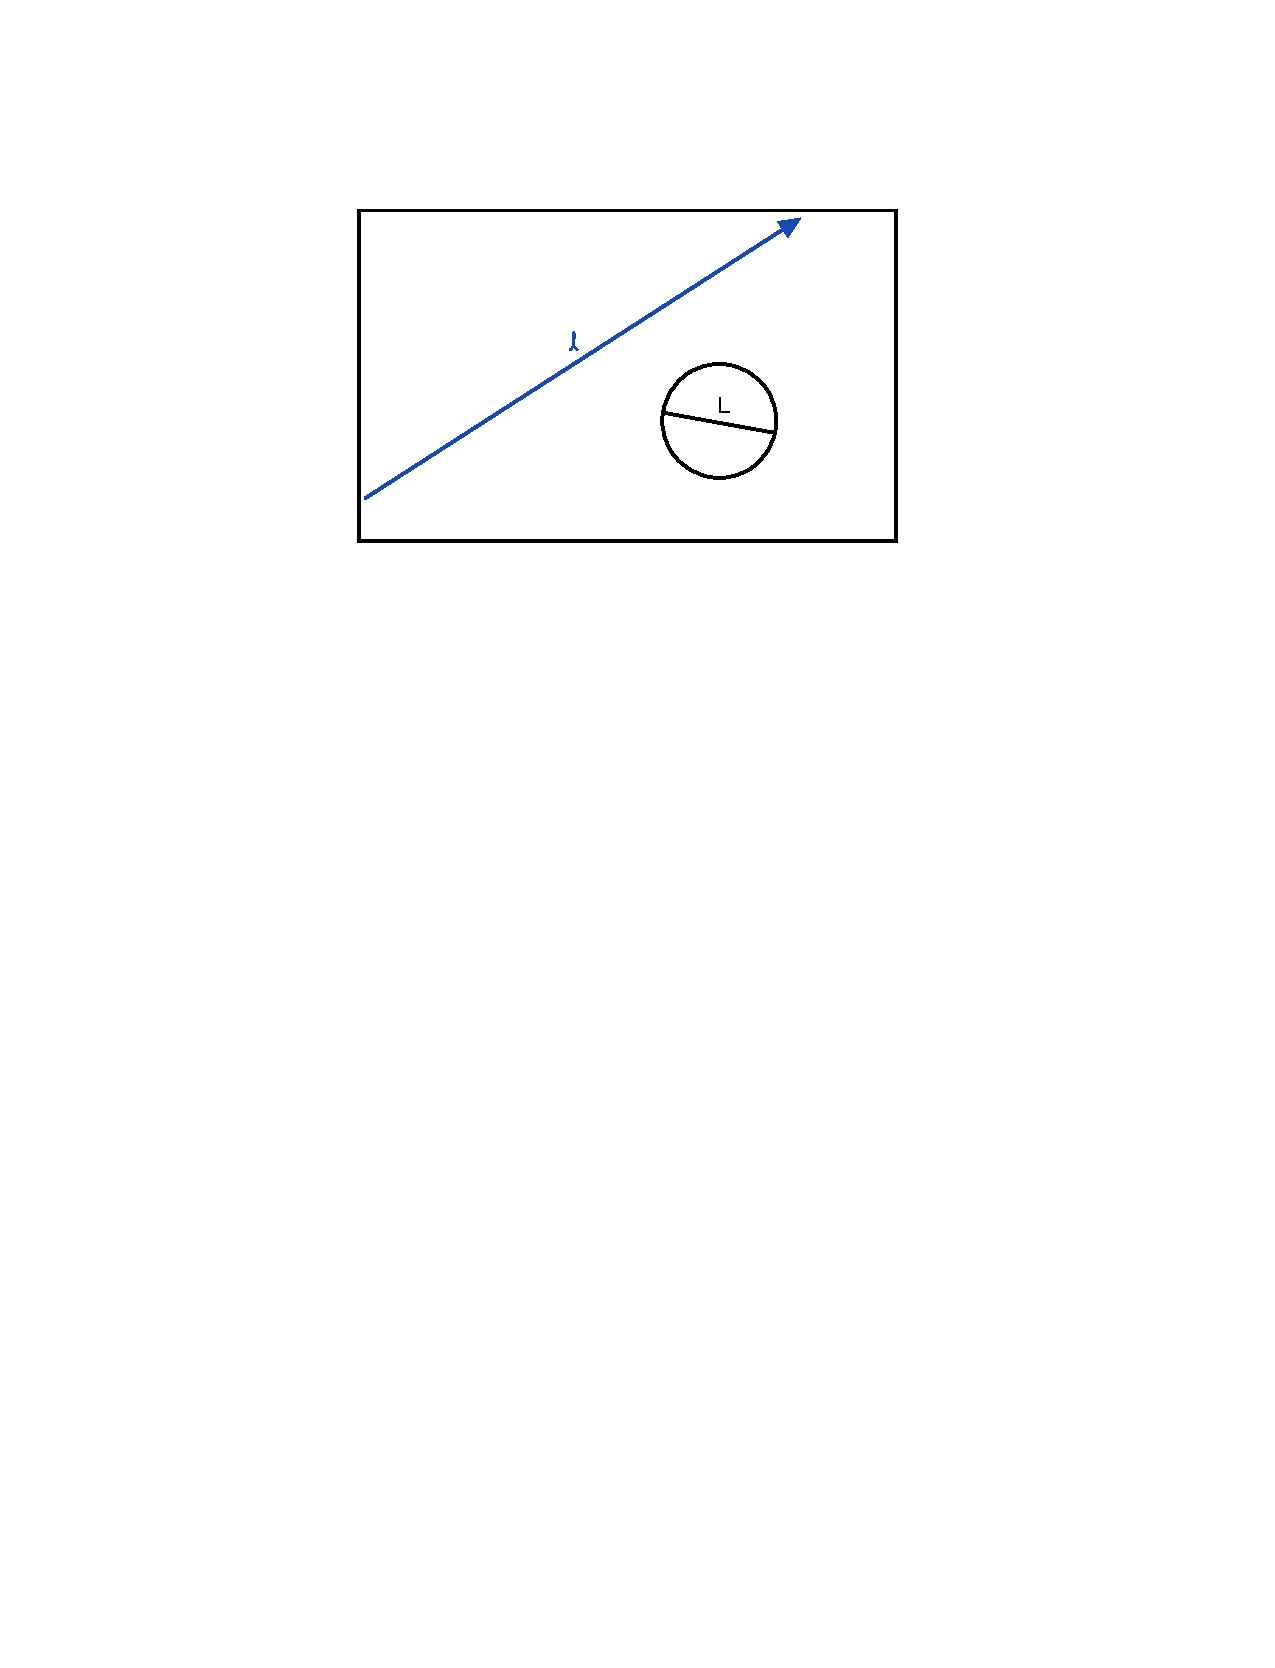
\includegraphics[scale=0.6]{figures/Large_Kn.pdf}
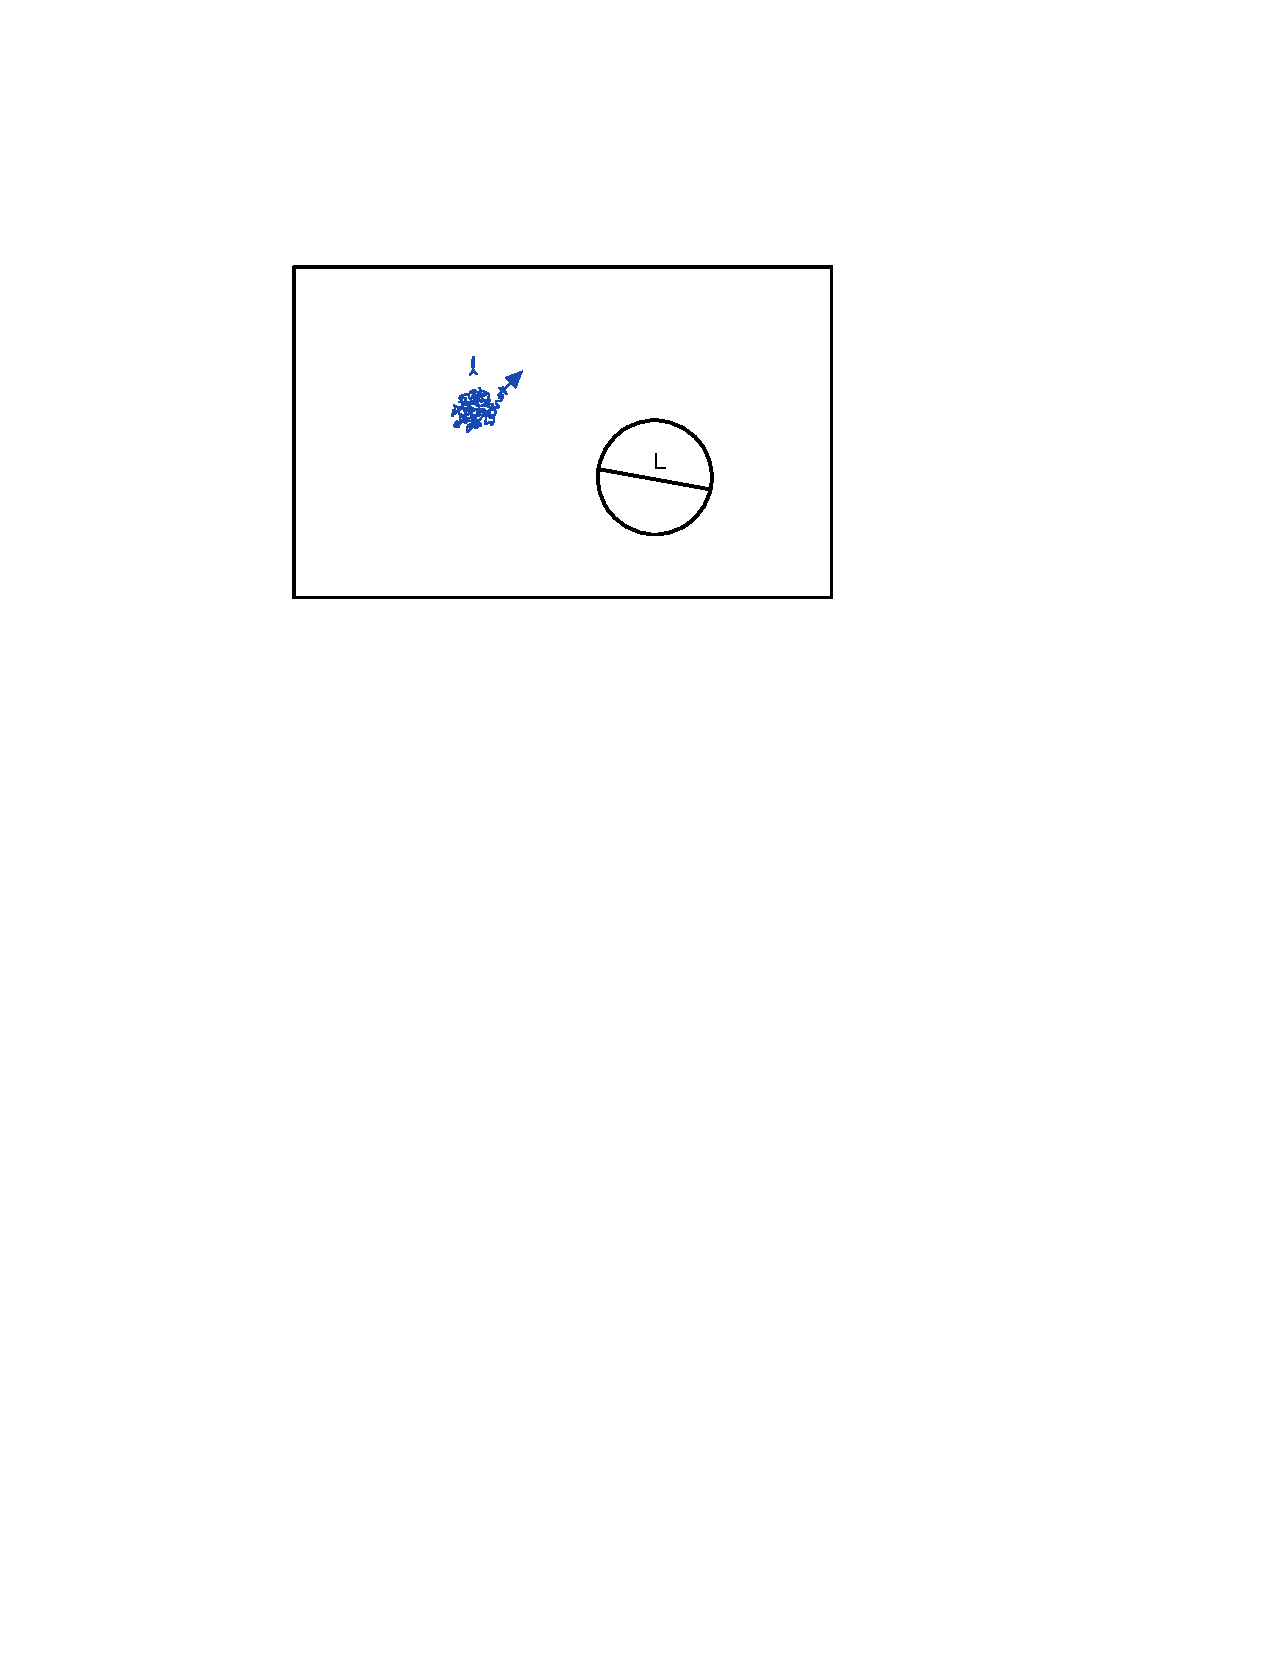
\includegraphics[scale=0.6]{figures/Small_Kn.pdf}
\end{center}
\caption{Characteristic length scale of problem, $L$, compared to mean free path of particles, $\ell$, for a flow with large Knudsen number (left) vs. small Knudsen number (right)}
\label{Knudsen_example}
\end{figure}

This work falls within the small Knudsen regime, so we will be working with the continuum description of fluids. In this section we will discuss the Navier-Stokes Equations that arise from this modeling technique and how we account for the supercritical nature of the flow through our choice of equation of state. 

\subsection{Continuum Description of Fluids}
The continuum hypothesis assumes that the fluid has no fine structures and that it is perfectly continuous, i.e. the properties of a small subdivision are the same as other subdivisions. This allows for the approximation of physical quantities at the infinitesimal limit \cite{cont}.

For example, consider a fluid with arbitrary volume $V$ as depicted in Figure \ref{cons_mass}.  

\begin{figure}[h!]
\begin{center}
\begin{tikzpicture}

% Blob
\path[draw, thick, scale=1.5, use Hobby shortcut, closed=true]
(0,0) .. (1,.4) .. (3,1) .. (4,.3) .. (2,-1.5) .. (.5,-1);
\path[draw,scale=1.5, use Hobby shortcut]
(1,.4) .. (1.2, -.425) .. (1,-1.25);
\path[draw, style=dashed, scale=1.5, use Hobby shortcut]
(1,.4) .. (.8, -.425) .. (1,-1.25);
\path[draw,scale=1.5, use Hobby shortcut]
(2,.77) .. (2.3, -.365) .. (2,-1.5);
\path[draw, style=dashed, scale=1.5, use Hobby shortcut]
(2,.77) .. (1.7, -.365) .. (2,-1.5);
\path[draw,scale=1.5, use Hobby shortcut]
(3,1) .. (3.4, -.18) .. (3,-1.36);
\path[draw,scale=1.5, style=dashed, use Hobby shortcut]
(3,1) .. (2.6, -.185) .. (3,-1.37);
%\path[draw, color=red, -stealth,scale=1.5, use Hobby shortcut, save Hobby path = {velocity}]
%(-.5,-.125) .. (0,0) .. (1,-.25) .. (2,-.5) .. (3,-.25) .. (4, 0) .. (4.5, -.125);
%\path[draw, color=red, yshift=1cm, -stealth,scale=1.5, use Hobby shortcut]
%(-.5,-.125) [ restore and use Hobby path={velocity}{}];
%\path[draw, color=red, yshift=-1cm, -stealth,scale=1.5, use Hobby shortcut]
%(-.5,-.125) [ restore and use Hobby path={velocity}{}];
%\fill (.7,-.3)  circle[radius=2pt] node[right]{A};
%\fill (3.8, -.3) circle[radius=2pt] node[right]{B};
\end{tikzpicture}
\end{center}
\caption{A fluid of arbitrary volume $V$ bounded by surface $S$ with velocity $\vec{v}(\vec{x},t)$. A differential volume and surface area is given by $dv$ and $ds$, respectively. $\vec{n}$ is the outward-pointing unit normal vector to the surface $S$.}
\label{cons_mass}
\end{figure}
For a fluid with density $\rho(\vec{x},t)$, mass within a small representative volume can be described with
$$ \rho \, dv$$
Total mass in the arbitrary volume is then given by 
$$\iiint_{V} \rho \,dv$$
The rate of change of mass through the volume is now 
$$\dfrac{d}{dt}\iiint_{V} \rho \, dv $$
\begin{equation} \label{volume_mass}
= \iiint_{V} \dfrac{\partial \rho}{\partial t}\,dv
\end{equation}
Simultaneously, overall change in mass throughout the volume can be described by the net mass flux through the surface $S$. Volumetric flow through a small portion of the bounding surface is given by
$$\vec{v}\cdot \vec{n} \, ds$$
Total mass flux through the entire surface is then
\begin{equation} \label{surface_flowthrough}
\iint_S \rho \, \vec{v}\cdot \vec{n} \, ds
\end{equation}
Applying the divergence theorem to Eq. \ref{surface_flowthrough} yields the following volume integral
\begin{equation} \label{volume_equiv}
\iiint_V \nabla \cdot \left(\rho \, \vec{v} \right) \, dv
\end{equation}
Assuming there is no additional source generating or leaking mass within the control volume, we can relate Eqs. \ref{volume_mass} to \ref{volume_equiv} : 
\begin{equation*}
\begin{aligned}
\iiint_{V} \dfrac{\partial \rho}{\partial t}\,dv &= - \iiint_V \nabla \cdot \left(\rho \, \vec{v} \right) \, dv \\ 
\iiint_{V} \dfrac{\partial \rho}{\partial t}\,dv &+ \iiint_V \nabla \cdot \left(\rho \, \vec{v} \right) \, dv  = 0 
\end{aligned}
\end{equation*}
\begin{equation} \label{cont_int}
\iiint_{V} \left( \dfrac{\partial \rho}{\partial t} + \nabla \cdot \left(\rho \, \vec{v} \right) \,\right) dv  = 0
\end{equation}
Note the inclusion of the negative sign for the right side of the initial equality; in the surface integral formulation, the outward facing normal describes flux out of the volume, thus yielding a decrease in mass within the volume. Since Eq. \ref{cont_int} holds for any arbitrary volume $V$, the integrand must be identically equal to zero:
\begin{equation} \label{conservation_mass}
\dfrac{\partial \rho}{\partial t} +  \nabla \cdot \left(\rho \, \vec{v} \right) \,  = 0
\end{equation}
Through the continuum hypothesis and conservation of mass, we have now arrived at the continuity equation in Eq. \ref{conservation_mass}. This specific process demonstrates an even more fundamental relationship known as a \textit{conservation law}. More generally, for some integrated property $\phi$, the rate of change of $\phi$ within a control volume must be equal to the amount of $\phi$ lost or gained through the boundaries of the control volume plus what is created or consumed by any sinks or sources, $s$, within the volume (sinks having positive orientation to match the positive orientation of the outward-facing normal $\vec{n}$) \cite{}. 
\begin{equation} \label{conservation_law}
\dfrac{\partial \phi}{\partial t} +  \nabla \cdot \left(\phi \, \vec{v} \right) + s \,  = 0
\end{equation}
In addition to this concept applying to conservation of mass, as was seen in this section, the idea outlined by Eq. \ref{conservation_law} applies to conservation of momentum and energy within the fluid. Together, these expressions combine to form the basis of the Navier-Stokes Equations, as will be seen in more detail in chapter 2. The important takeaway from this section is that with the continuum hypothesis and fundamental laws of physics, one can adequately capture macroscopic flow behavior for the types of flows we are interested in within this work.  

\subsection{Equation of State}
Conservation of mass, momentum, and energy gives us five equations to describe our fluid system. For compressible flows, this is not enough information to solve for all the unknowns within the system of coupled partial differential equations. A sixth equation, known as the \gls{eos}, must be chosen in order to close the system. The \gls{eos} relates three of the six unknowns: pressure, temperature, and density. Here we will briefly discuss some \gls{eos} options and their distinguishing characteristics in order to motivate the choice made for this work. 

The simplest option available is the ideal gas \gls{eos}, which comes from the ideal gas law. This \gls{eos} relates density, pressure, and temperature in the following manner: 
\begin{equation} \label{ideal_gas}
p = \dfrac{RT}{V_m}
\end{equation}
where $p$ is pressure, $R$ is the universal gas constant, $T$ is temperature, and $V_m = \tfrac{V}{n}$ is the molar volume of the fluid (it is common to express density in terms of molar volume for sake of simplicity in writing the \gls{eos} with $V$ being volume and $n$ being the number of moles). The ideal gas \gls{eos} is fairly accurate for liquids and gases at moderate temperatures and low pressures. It fails at low temperatures and high pressures, especially near the transition region from gas to liquid. The inaccuracy noted in this region means this \gls{eos} would not be suitable for the area of interest within this study. 

Cubic \gls{eos} generally provide more accuracy than the ideal gas \gls{eos}. The first cubic \gls{eos} was developed by van der Waal in 1873, modifying the ideal gas \gls{eos} to take into consideration the finite size of molecules and interactions between molecules (the ideal gas \gls{eos} only accounts for interactions with the container and treats molecules as point particles). Other cubic \gls{eos} can be thought of as modifications from this base form: 
\begin{equation} \label{vanderwaal}
p = \dfrac{RT}{V_m - b} - \dfrac{a}{V_m^2}
\end{equation}
where $a$ and $b$ are constants related to the pressure and temperature at the critical point, $p_c$ and $T_c$ respectively: 
$$a = \dfrac{27(RT_c)^2}{64p_c}\,, \quad b = \dfrac{RT_c}{8p_c}$$
One of the main benefits of using a cubic \gls{eos} is that they can have comparable and sometimes even better accuracy compared to their higher order counterparts, thus reducing computational costs. However, it is important to take into consideration the regime of interest in addition to the fluid of interest when choosing an \gls{eos}, as each one has its own pros and cons. For example, molecule polarity and density are two factors that can have a high impact in selection between the \gls{srk} and \gls{pr} alone \cite{GHANBARI201713}. 

This work uses the \gls{srk} as will be more thoroughly introduced in chapter 2. It has been shown that this equation of state is fairly accurate for the parameter regime under careful consideration in this work \cite{}. This accuracy is detailed further in chapter 3 through comparisons with data from \gls{nist}. Overall, when adequately considered, the \gls{eos} is the key avenue to incorporating specific fluid properties into the mathematical model.


\section{Turbulence}
In addition to the categorizing of fluid type, fluid flow can be distinguished into different types based on certain defining flow characteristics. The main two classifications of note are laminar flow and turbulent flow.

Laminar flow is denoted by fluid particles having well-defined parallel trajectories of motion, or streamlines. Streamlines do not cross, meaning adjacent layers within the fluid flow by one another with little to no mixing. From a more generalized perspective, the flow appears to be smooth. In contrast to this, turbulent flow is characterized by its unpredictable and chaotic trajectories. Streamlines do cross resulting in swirls and eddies of varying length scales which induce mixing. Turbulent flow can be qualitatively described as being rough due to this high degree of fluctuation within the velocity and pressure fields present. This generalized description is depicted in Figure \ref{lam_vs_turb}.

\begin{figure}[h!]
\begin{center}
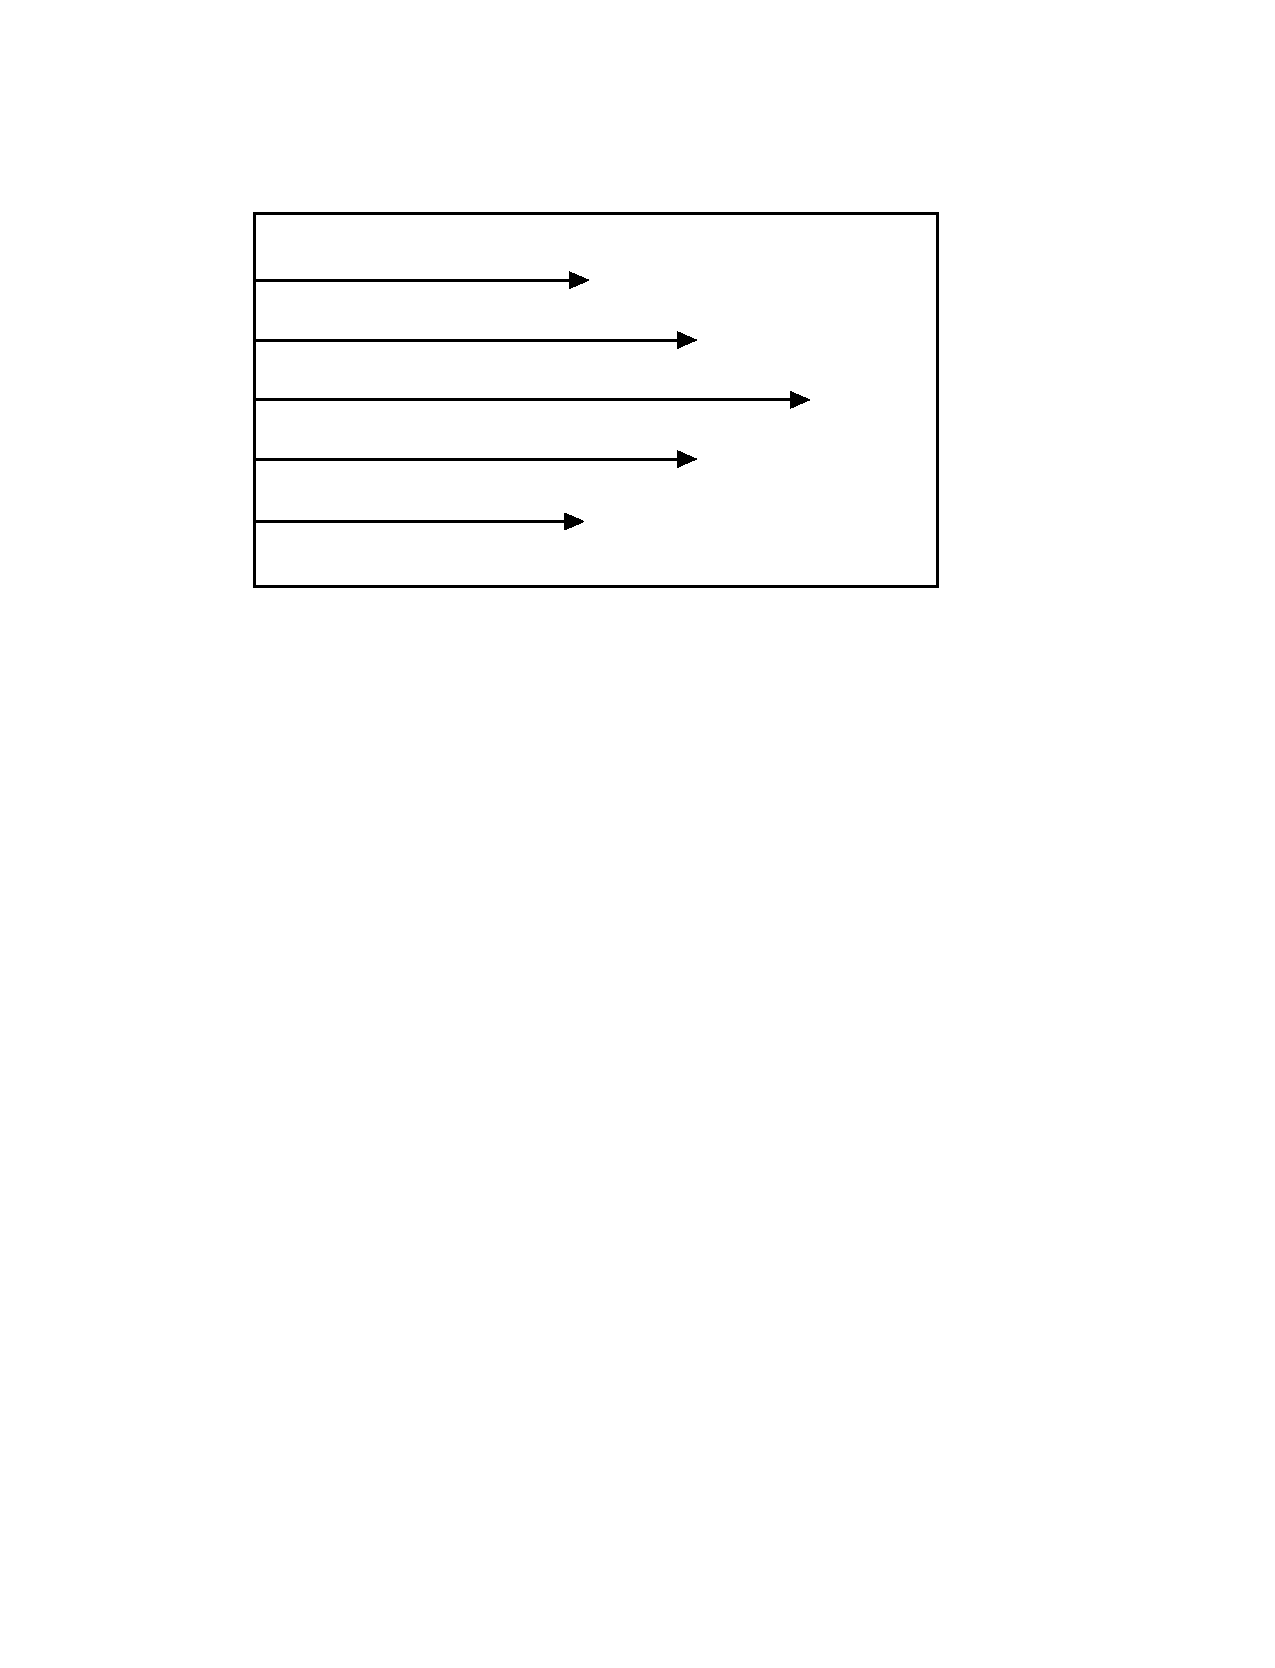
\includegraphics[scale=0.5]{figures/laminar}
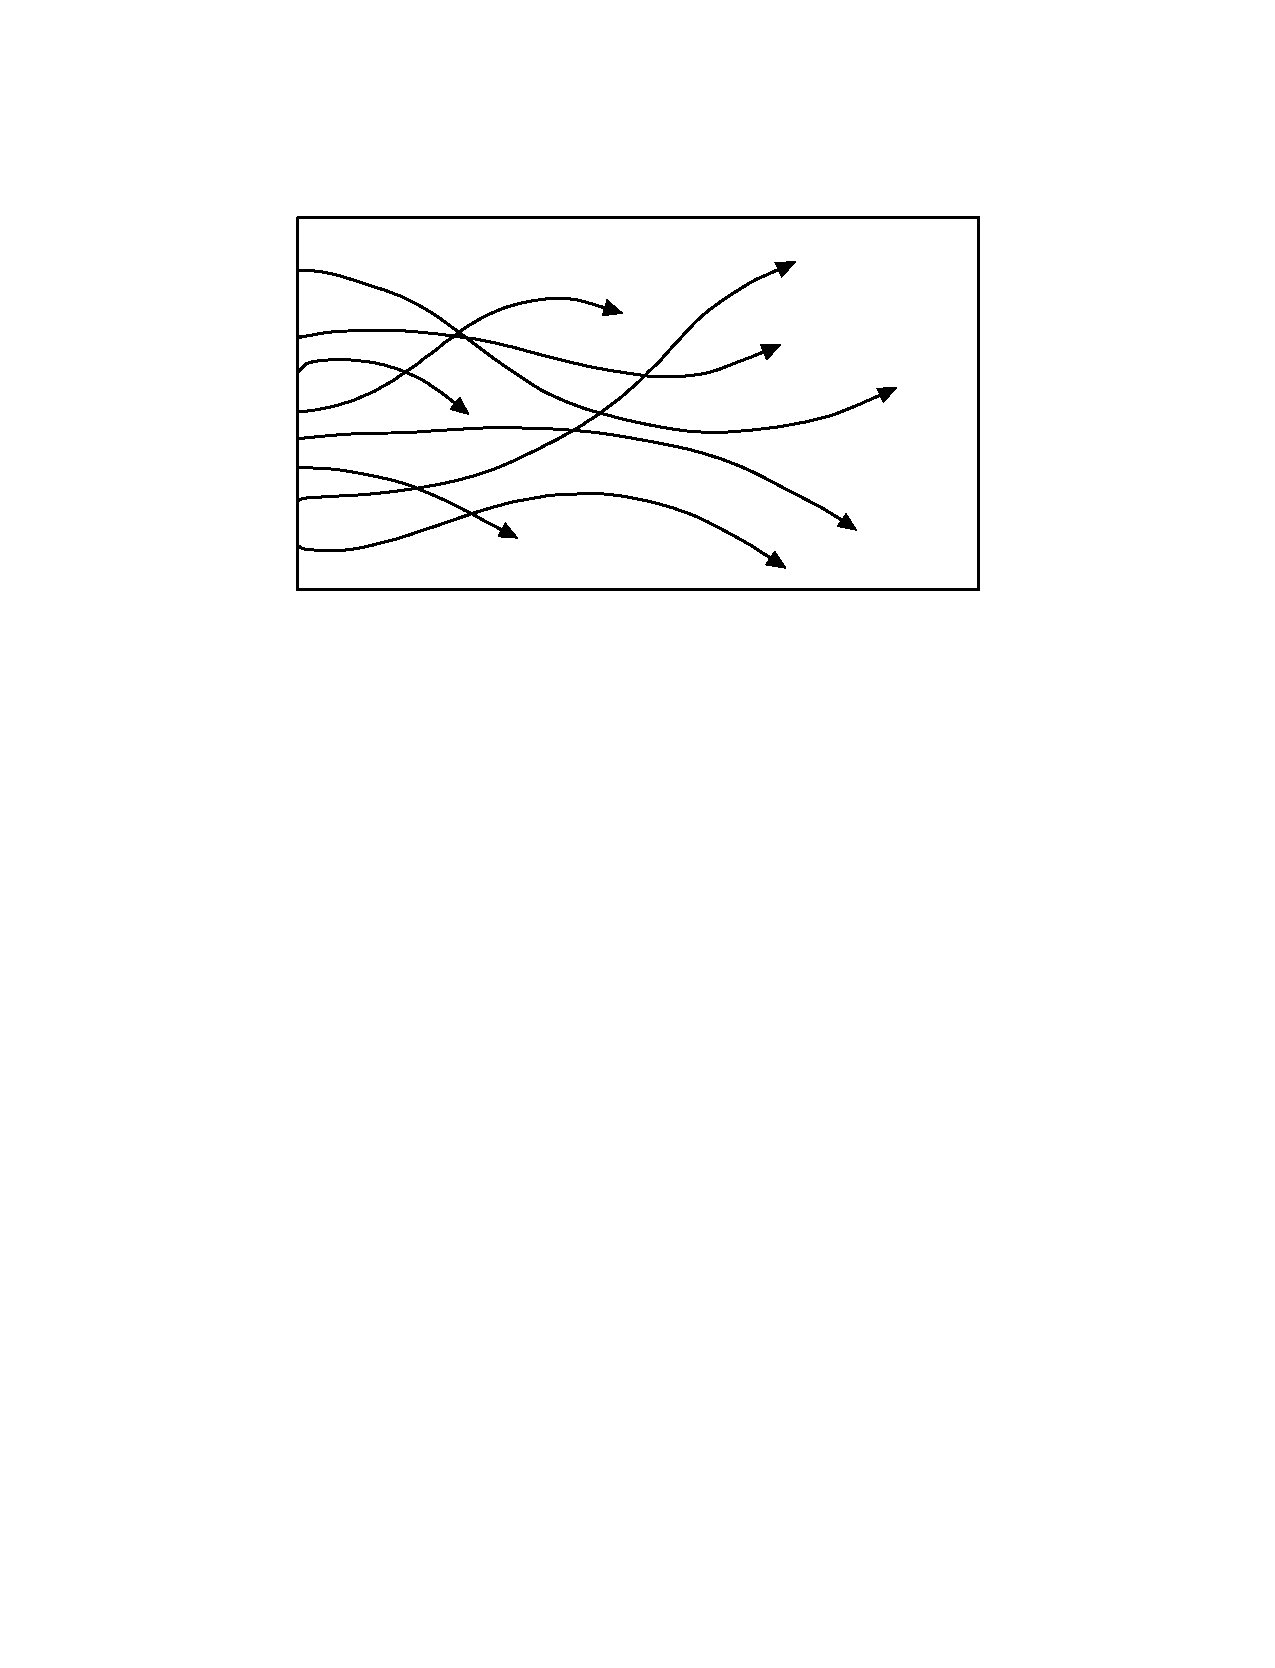
\includegraphics[scale=0.503]{figures/turbulent}
\end{center}
\caption{Example of streamlines in laminar (left) vs. turbulent (right) flow.}
\label{lam_vs_turb}
\end{figure}

The Reynolds number is a dimensionless value that can be used to distinguish laminar flow from turbulent flow. It is defined as follows:
\begin{equation}
\label{Reynolds_num}
\text{Re} = \frac{\rho u L}{\mu}
\end{equation}

\noindent where $\rho$ and $\mu$ are the density and dynamic viscosity of the fluid, respectively, $u$ is the flow velocity, and $L$ is a characteristic length scale associated with the given flow scenario (e.g. pipe diameter). As is demonstrated by the ratio in Equation \ref{Reynolds_num}, the Reynolds number measures the relative effects of inertial forces compared to viscous forces within a given flow scenario. A small Reynolds number signifies the dominance of viscous forces; fluid parcels moving in tandem want to ``stick together," resulting in the sheared flow and parallel trajectories seen in laminar flow. Turbulence is then characterized by a large Reynolds number, where inertial forces take precedence. Here, deviations within the laminar flow field result in lateral mixing between shear layers. This creates eddies and random trajectories that result in the chaotic motion of turbulent flow. 

This work focuses on the turbulent round jet and its associated dynamics in the context of supercritical fluids. The remainder of this section details a brief historical overview of turbulence modeling and numerical methods developed for studying turbulence in order to motivate the modeling and numerical choices made within this work.

\subsection{Historical Perspective}
This is a brief history of turbulence study from a mathematics perspective.


\subsection{Numerical Approaches}
These are some of the numerical approaches in use, including what we use and why we use it. 
\begin{figure}[h!]
\begin{center}
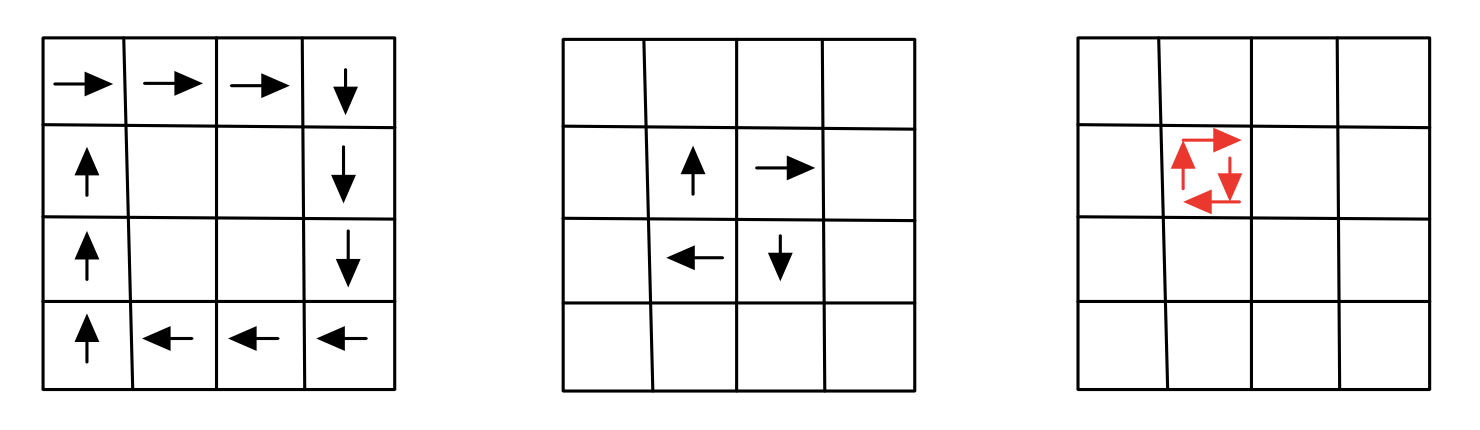
\includegraphics[scale=0.5]{figures/LES_grid}
\end{center}
\caption{LES resolves large scale eddies (black) and models fine scale eddies that are unresolved due to mesh size (red).}
\label{LES_grid}
\end{figure}

\section{Supercritical Carbon Dioxide}
As mentioned earlier, supercritical fluids have many qualities that make them desirable as working fluids in a variety of systems. We now shift our focus to one particular fluid of interest: \gls{co2}. As seen in the phase diagram of Figure \ref{phase_diagram}, the critical temperature, $T_c$, and critical pressure, $p_c$, of \gls{co2} are $304.128 $ K and $73.773$ bar. The critical temperature and pressure of \gls{co2} is fairly easy to attain, making it a strong candidate for systems with hight thermal outputs. Additionally, \gls{sco2} has a relatively low toxicity and environmental impact \cite{}, and is chemically stable, non-flammable, and readily available \cite{}. For these reasons, \gls{sco2} is a highly coveted alternative working fluid in many different applications, and is one of the most widely used supercritical fluids along with water \cite{SCF2}. 

\begin{figure}[h!]
\begin{center}
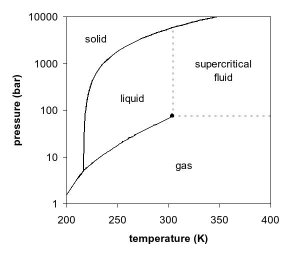
\includegraphics[scale=.75]{figures/co2_phase_diagram}
\end{center}
\caption{Phase diagram for Carbon Dioxide (CO2). Critical pressure, $p_c$, and temperature, $T_c$, are $73.773$ bar and $304.128$ K, respectively.}
\label{phase_diagram}
\end{figure}

In the next part of this section, we will explore some applications of \gls{sco2} in which the turbulent round jet configuration is used. Then we will go through a brief review of recent studies involving \gls{sco2}, and more generally supercritical turbulent jets, in order to demonstrate where this work fits in among current research. Finally, we outline the structure of the remainder of the dissertation. 

\subsection{Applications of Interest}
One of the key applications of interest that motivates this work is the use of \gls{sco2} as the working fluid in advanced cycles for power generation. \gls{sco2} has shown promise as a working fluid for both indirect cycle and direct-firing cycles \cite{WEILAND2017293, WHITE2021116447}. One example of indirect cycle improvement uses \gls{sco2} in place of water for the conventional steam-Rankine cycle. An example of where these types of configurations may prove useful is in managing thermal runoff from existing coal and natural gas combustion processes \cite{WEILAND2017293}. Compared to steam, \gls{sco2} is less corrosive, more thermally stable, and has increased power density. The critical point of \gls{co2} is easily accessible, and once achieved, allows for the use of a single phase fluid design, leading to a simplified and more compact turbine (see Figure \ref{turbine_comp}). Ultimately, this also allows for lower operation and maintenance costs \cite{Dodge}. The benefits of using sCO2 turbines over the traditional steam design has been highly researched and has only seen an increase in momentum for implementation \cite{CRESPI2017152, NextGenNucReac, hitthemarket, commercialization}. 

\begin{figure}[h!]
\begin{center}

\includegraphics[scale=.5]{figures/steam_vs_sco2_turbine}
\end{center}
\caption{Size comparison for steam vs. \gls{sco2} turbine via Echogen Power Systems LLC \cite{commercialization}.}
\label{turbine_comp}
\end{figure}

An example of direct-firing cycles that use \gls{sco2} include the Allam cycle \cite{allam2013system}. When compared to the conventional Brayton cycle, studies show that the Allam cycle has much higher efficiency \cite{ALLAMCOMP, ALLAM20175948}. Additionally, the carbon footprint for the Allam cycle is virtually zero, allowing for \gls{co2} produced from the system to be stored underground or used elsewhere, aiding in carbon sequestration efforts \cite{cleantechnol1010022}. This two-for-one benefit of using \gls{sco2}-based cycles such as the Allam cycle has spurned much research \cite{ALLAMTech1, CHAN2021113972} and development \cite{8Rivers} into related technologies.

Of particular importance to these applications is the round turbulent jet, as this is a major component of many injection technologies. The high densities associated with the liquid-like aspect of supercritical fluids coupled with the relatively low gas-like viscosity associated with them typically results in a high Reynolds flow, often resulting in a turbulent system. The turbulence physics of these jets is crucial in developing machinery for these systems. Current experimental research is mainly application oriented. Research into the \gls{sco2} jet's rock breaking ability has been of primary importance to \gls{egs} applications \cite{EGScomp, EGS2, very_rock, experiment, rb}, with additional focus being given to pipeline leakage and flow dynamics upon wall impact \cite{WANG2015210, WANG201977}, which unfortunately does not explore the underlying turbulence statistics of the flow. Chemical engineering design aspects of \gls{sco2} injection are more focused on solubility dynamics as opposed to turbulence \cite{freejet, pulse_jet}. Other experiments focus on similar application specific quantities of interest, such as heat transfer and mixing, which is related in part to the turbulence dynamics \cite{heated_cyl}, but they also note the difficulty in experimental design for investigating these aspects of the flow under the conditions needed to replicate those in real applications \cite{freejet}. Thus, numerical simulations are necessary to further explore the turbulence statistics of these flows.


\subsection{Overview of Current Numerical Landscape}
Much research has gone into the development of appropriate numerical methods for such investigations, though challenges arise due to the lack of experimental data for use in model validation. Studies using \gls{dns} have been implemented to help establish benchmark test cases for other types of numerical schemes. Ruiz et al. use 2D \gls{dns} to simulate a mixing layer created by two streams of supercritical Oxygen and gaseous Nitrogen, using two different \gls{cfd} solvers to add confidence to their results \cite{article}. A 3D \gls{dns} is used by Ries at al. to simulate a round Nitrogen jet for comparison with experimental data produced by Mayer et al. \cite{DNS_N}. However, this study requires a reduction in Reynolds number from $1.62 \times 10^5$, based on the injection diameter, to $5300$ in order to feasibly execute the computations. Li also utilizes a low Reynolds number of $1750$ to study a round turbulent \gls{sco2} jet with a preconditioning scheme \cite{Li2012}. The \gls{rans} approach has also been implemented utilizing theory from the ideal gas case \cite{RANS}, but with the goal of ascertaining a more general understanding of why specifically \gls{sco2}'s rock-breaking ability is better than that of water. 

In order to maintain a high Reynolds flow and better capture the effects of the supercritical nature of the fluid on the turbulence dynamics, the use of \gls{les} has been explored. The impact of \gls{sgs} models in capturing transcritical and supercritical dynamics of cryogenic Nitrogen have been analyzed through comparison with the Mayer et al. experiment and highly accurate \gls{nist} data \cite{PETIT201361, doi:10.1080/00102200500287613, doi:10.1063/1.1795011, doi:10.1063/1.4937948, Same_LES}. Schmitt et al. does a similar investigation using \gls{les}, then extending their investigation to include \gls{sco2} after validation with the Mayer et al. data. \cite{LES_N} However, this investigation uses low-pressure jets and does note the \gls{sgs} models might need additional contributions to handle non-linearities and the pressure regime. While many of these investigations note that \gls{sgs} models may need modification to deal with supercritical flows \cite{LES_N, PETIT201361, doi:10.1063/1.4937948, doi:10.1080/00102200500287613}, it is noted by Muller et al. that given a sufficiently fine grid, the influence of \gls{sgs} modeling and numerical flux discretization is essentially limited to second-order moments \cite{doi:10.1063/1.4937948}. Thus, we will be using the compressible version of the dynamic Smagorinksy \gls{sgs} closures for our investigation, with further consideration of any influence of \gls{sgs} model on our quantities of interest being noted later on. 

While much of the literature thus far has explored the impact of different numerical methods on modeling supercritical fluid flows and has aimed to strengthen the validity of these simulations in spite of the lack of experimental data available in the current landscape, a general consensus has still not been reached on how the supercritical nature of these fluids impacts the turbulence physics of these models. Thus, there remain open questions for understanding the fundamental flow behavior of turbulent jets in a supercritical environment, especially near the supercritical point, where both experimental and numerical investigations are still a challenge.

Our objective is to use \gls{les} to investigate the turbulence physics of \gls{sco2} near the critical point in order to capture the effects of widely varying thermal properties of supercritical fluids. Using the compressible Navier-Stokes equation solver, \textit{PeleC} \cite{osti_1374142}, closed with the \gls{srk}, we consider three cases in order to examine various quantities of interest associated with classical turbulence mechanics. These three cases are chosen to capture different areas around a peak in specific heat that is associated with the pseudo-critical region. The rest of the paper is as follows. We first present the physical model and numerical methods used for the investigation. We then present the simulation setup of the round turbulent jet as implemented in the code. Next we present the results of the turbulent \gls{sco2} jet and our analysis of the turbulence statistics. 





